\documentclass[12pt]{third-rep}

%% This skeleton report is organised as a master file called
%% report.tex which then includes files for individual parts including
%% abstract.tex, chapter1.tex, chapter2.tex, chapter3.tex and
%% appendix1.tex.  

\usepackage{url} % typeset URL's sensibly
\usepackage{pslatex} % Use Postscript fonts
\usepackage{listings}
\usepackage{amsmath}
\usepackage{graphicx}
\graphicspath{{images/}}
\usepackage{parskip}
\usepackage{fancyhdr}
\usepackage{vmargin}
\usepackage{multicol}
\usepackage{array}
\usepackage[table,xcdraw]{xcolor}
\usepackage{pdflscape}
\usepackage{fancyvrb}
\usepackage{tikz}
\usepackage{caption}
\usepackage{rotating}
\usepackage{hyperref}

%% This defines the title (the \\ forces a line break)
\title{CogniDriver}
%% and author
\author{Maria - Daniela Florescu}
%% and supervisor
\supervisor{Dr. Toby L. J. Howard}
%% and the year of the report
\reportyear{2015}

\makeatletter
\let\thetitle\@title
\let\theauthor\@author
\let\thedate\@reportyear
\makeatother

\pagestyle{fancy}
\fancyhf{}
\rhead{\theauthor}
\lhead{\thetitle}
\cfoot{\thepage}

%% this defines the file that contains the text of the abstract, there
%% must be one of these by the time you submit your report.
\abstractfile{abstract.tex}

%% this defines the file that contains the acknowledgements (it can be
%% omitted if you don't feel like thanking anyone
\thanksfile{merci.tex}

%% End of preamble, the actual document starts here
%%

\begin{document}

\begin{titlepage}
	\centering
    \vspace*{0.5 cm}
    
\includegraphics[scale = 0.50]{crestbw.png}\\[1.0 cm]	% University Logo
    \textsc{\LARGE The University of Manchester}\\[2.0 cm]	% University Name
	\rule{\linewidth}{0.2 mm} \\[0.4 cm]
	{ \LARGE \bfseries \thetitle}\\
	\rule{\linewidth}{0.2 mm} \\[1.5 cm]
	
	\begin{minipage}{0.4\textwidth}
		\begin{flushleft} \large
			\emph{Author:}\\
			\theauthor
			\end{flushleft}
			\end{minipage}~
			\begin{minipage}{0.4\textwidth}
			\begin{flushright} \large
			\emph{Supervisor:} \\
			Toby L. J. Howard					
		\end{flushright}
	\end{minipage}\\[2 cm]
	
	{\large \thedate}\\[2 cm]
 
	\vfill
	
\end{titlepage}

%% This actually creates the abstract page
\vspace*{\fill}

\begin{center}
	\Large
	\vspace{0.9cm}
    \textbf{Abstract}
    
    CogniDriver
    
    Author: Maria - Daniela Florescu    
\end{center}

The aim of the project is to provide an overview of the development of CogniDriver, a 3D mind-controlled car driving game which uses the Emotiv EPOC interface to control the car movement. The headset also allows the activation of various game effects such as raining when the frustration levels are too high or changing the camera view when the player does a left wink.

The Unity game engine has been used while developing the game in order to gain access to an advanced physics engine and to a multi-platform deployment tool.

The results of user testing on 13 participants have shown that although it is more difficult to control the game while in Cognitiv mode, the game appears more challenging and more interactive than a normal Keyboard mode play. 

In the conclusions, a short overview of the current deficiencies are presented as well as potential for further development.

\begin{center}  
	\Large  
    Supervisor: Toby L. J. Howard
\end{center}

\vspace*{\fill}
\vspace*{\fill}

\begin{center}
    \textbf{Acknowledgements}   
\end{center}

I would firstly like to thank my supervisor, Toby Howard, who has provided great advice and support throughout the project. 

I would also like to thank my family for their continuous support during my studies.

Finally, a big thank you to everyone who has helped with testing this project and whose feedback was greatly appreciated.

\vspace*{\fill}

%% Generate contents etc
\tableofcontents
\listoffigures
\listoftables

\pagestyle{fancy}
\renewcommand{\chaptermark}[1]{ \markboth{#1}{} }
\renewcommand{\sectionmark}[1]{ \markright{#1}{} }
\fancyhf{}
\fancyhead[LE,RO]{\slshape \rightmark}
\fancyhead[LO,RE]{\slshape \leftmark}
\fancyfoot[C]{\thepage}

%% These include the actual text
\chapter{Introduction}
\label{cha:intro}

\section{Applications}

Using BCI (Brain Computer Interfaces) to control an application is of great use to persons with motor disabilities whose use of keyboard or mouse devices might not be convenient. In addition,  BCIs provide a great way to exercising brain functions and improving concentration.

\section{Aims and objectives}

The aim of this project was to learn about the ... and falls of BCIs, how these interact with the computer and reach a conclusion about how they could be used in the future. Because the Emotiv EPOC Control Panel allows only up to 4 actions to be recognised at any one time, the simplest choice of a game was that of a car driving one since you can also observe the car moving in the dictated direction which can ease the activation of an action through the visual feedback.

The key objectives of the project were to:
\begin{itemize}
	\item Allow the car to move in each one of the four directions: forward, back, left, right through keyboard use; 
	\item Reach access to the interpreted data of the developers' SDK;
	\item Allow players to train new profiles inside the game;
	\item Provide an array of cars and colours that the user can select from.
\end{itemize}

\section{Report outline}

The report begins with describing the used tools and provides some information about the way the brain works in Chapter 2. Next, Chapter 3 describes how the Emotiv EPOC works and how it is organised. In this chapter, the report also contains a quick look over some other applications developed with this technology.

Chapter 4 focuses on the description of the design of this project, while Chapter 5 oversees the implementation details. Chapter 6 reviews the obtained results, while Chapter 7 described the performed testing. Appendix 1 shows the user questionnaire used during the user trials. Finally, Chapter 8 contains the conclusions of this project.
\chapter{Background}
\label{cha:background}

This chapter aims to provide a general overview of the tools used while building CogniDriver. It also describes some basic concepts about how the brain works which would be useful to know before diving into the description of the headset. 

\section{Development tools}

\subsection{Unity}
Unity is a game engine which allows:
\begin{multicols}{2}
\begin{itemize}
	\setlength\itemsep{-2mm}
	\item Game deployment on a variety of platforms;
	\item Easy object importing;
	\item Object manipulation;
	\item Scene design;
	\item Creation of primitive shapes (spheres, cubes, etc.);
	\item Collision detection;
	\item Automatic object updates;
	\item Game physics.
\end{itemize} 
\end{multicols}

I should also highlight some of the reasons why Unity was chosen in favour of other game engines such as UnReal. Unity allows file import by a simple drag-and-drop and it also auto-updates the objects if the source files are changed using another program (e.g. Paint, Photoshop). The advantages of UnReal over Unity would be better graphics (mainly lighting) and the fact that it can fracture meshes. In terms of scripting, Unity allows development in JavaScript, C\# and Boo, while UDK only allows UnrealScript. For CogniDriver, C\# has been the scripting language choice, because it allows Object Oriented Programming (OOP), it is scalable for larger projects and bugs are easier to track down. 

Unity has been used to create games such as Assassin's Creed Identity, Need for Speed World and Battlestar Galactica Online.

\subsection{Easy Roads 3D}
This plugin is available in the Unity asset store. The free version has been used for this project. It allows placing markers through which the road should go, and given a specified width, it approximates corners and builds the rest of the road into a single layer.

\subsection{Photoshop}
A trial version has been used to create some materials and textures such as: skid marks, rain, smoke texture, speedometer, arrows, colours choice. None of these are difficult to create, but I like Photoshop because it is easy to use by both novice and professional users. In addition, the layers allow the user to create many compositions and modify the image at will.

\section{Electroencephalography (EEG)}
The neuron is the core component of the nervous system. More neurons can connect together to form synapses and when one of these cells is excited, an electrical signal is generated. The electrical signals can be amplified and the resulting waveforms, known as brainwaves, can thus be obtained. They can then be used to monitor the brain activity of a person in order to detect abnormalities. In table \ref{table:brainwaves}, a representation of each type of most common brainwave types is shown, together with the normal activities in which these occur most often. 

\begin{table}[h]
\newcolumntype{C}{>{\centering\arraybackslash} m{2cm} }  %# New column type
                             
\begin{tabular}{ | C | C | C | m{8cm}C | }
\hline
\textbf{Name}  & \textbf{Frequency (Hz)} & \textbf{Occurs in} & \textbf{Image Representation} \\ \hline
Delta & \textless 4    & deep sleep , unconsciousness, deep anaesthesia, \gls{hypoxia}          & 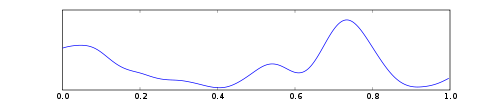
\includegraphics[scale=0.5]{500px-Eeg_delta.png}        \\ \hline
Theta & 4 - 7          & stress, unconsciousness, deep relaxation          & 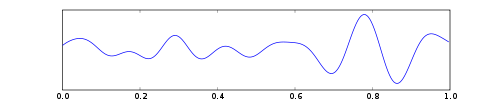
\includegraphics[scale=0.5]{500px-Eeg_theta.png}        \\ \hline
Alpha & 8 - 15         & relaxation          & 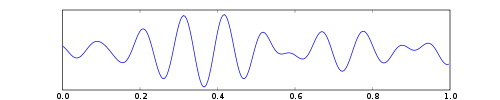
\includegraphics[scale=0.5]{500px-Eeg_alpha.png}        \\ \hline
Beta  & 16 - 31        & conciousness, alertness, thinking, sensory stimulation          & 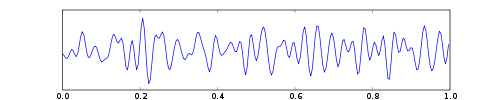
\includegraphics[scale=0.5]{500px-Eeg_beta.png}         \\ \hline
Gamma & 32 +           & selective attention, human cognition and perceptive activities         & 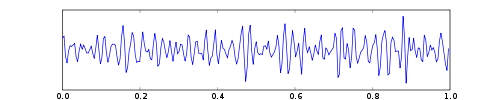
\includegraphics[scale=0.5]{500px-Eeg_gamma.png}        \\ \hline
\end{tabular}
\caption {Information about brainwaves types \cite{musicEEG}. Image Credit: Hugo Gamboa}
\label{table:brainwaves}
\end{table}

\begin{figure}
  \centering
  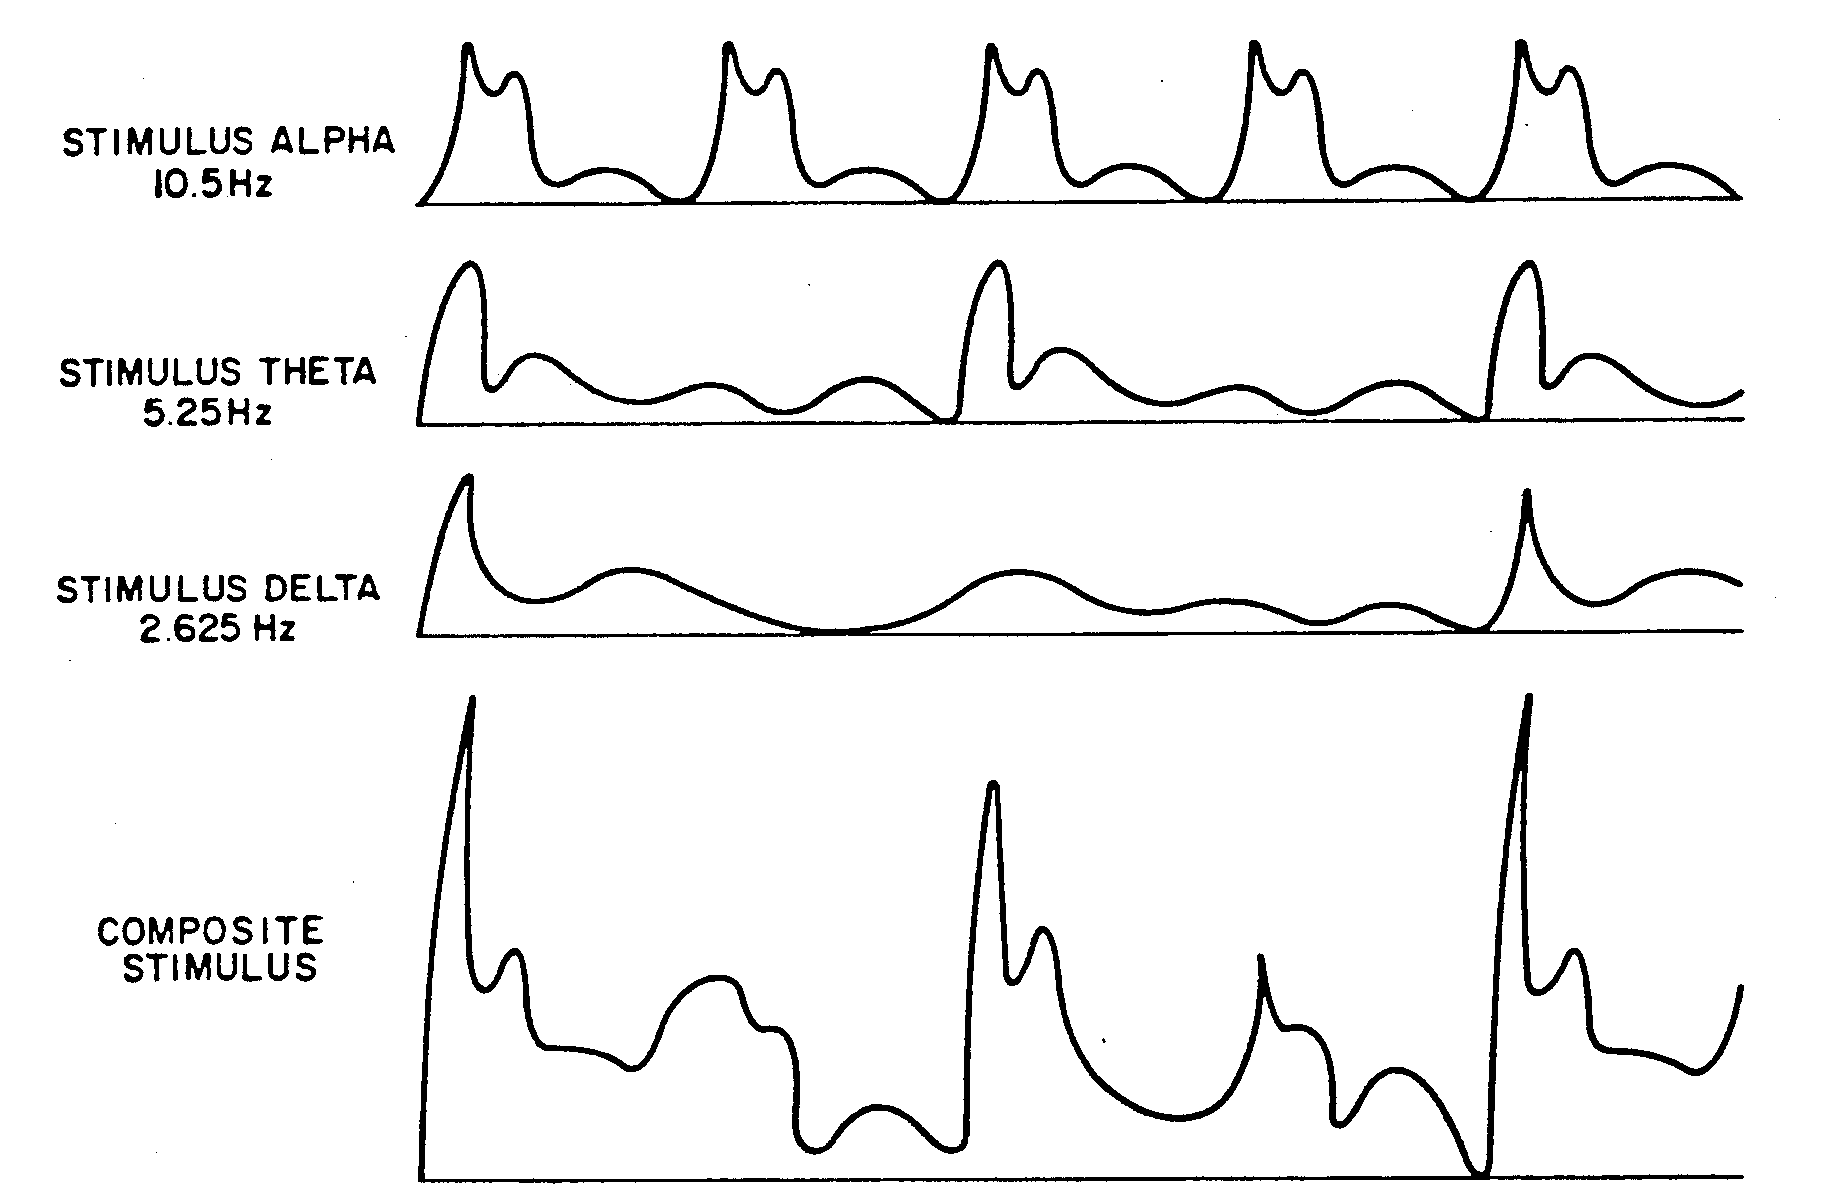
\includegraphics[width=350px]{BrainwaveComposition.png}
  \caption{A composition of alpha, theta and delta brainwaves. Credit: \cite{gall1992method}}
    \label{fig:brainwaveComposition}        
\end{figure}

Please note that almost always the EEG will display a composition of a set of types at any point in time. One example can be seen in the figure \ref{fig:brainwaveComposition}. Brain Computer Interfaces (BCIs) are a channel of communication between the electroencephalograph (EEG) and the computer.


\chapter{Introducing the Emotiv EPOC}
\label{cha:epoc}

\section{SDK description}
The Emotiv EPOC headset is a portable EEG device which consists of 14 sensors that transmit raw EEG data (see figure \ref{fig:sensorPos} for their positioning) to the computer and 2 reference sensors (CMS - Common Mode Sense and DRL - Driven Right Leg). The CMS sensor is the point on the scalp against which everything else is measured. The DRL sensor provides a feedback signal to cancel common mode noise in the electronics \cite{refSensors1, refSensors2}. See table \ref{table:sensorName} for the meaning of the abbreviations of sensor positions. The raw data gets interpreted and the user gains access to all of the information in one of the following 4 suites: Expressiv, Affectiv, Cognitiv, Mouse Emulator. 

\begin{figure}
  \centering
  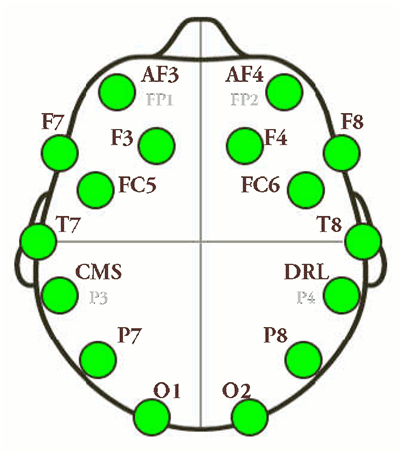
\includegraphics[width=250px]{sensorPositioning.png}
  \caption{Sensor positioning for the Emotiv EPOC. Credit: Emotiv}
    \label{fig:sensorPos}           
\end{figure}

\begin{table}[h]
\centering
\begin{tabular}{|c|c|llcc}
\cline{1-2} \cline{5-6}
\textbf{Abbreviation} & \textbf{Meaning} &  & \multicolumn{1}{l|}{} & \multicolumn{1}{c|}{\textbf{Colour code}}          & \multicolumn{1}{c|}{\textbf{Meaning}} \\ \cline{1-2} \cline{5-6} 
A                     & Ante             &  & \multicolumn{1}{l|}{} & \multicolumn{1}{c|}{Black}                         & \multicolumn{1}{c|}{No signal}        \\ \cline{1-2} \cline{5-6} 
F                     & Frontal          &  & \multicolumn{1}{l|}{} & \multicolumn{1}{c|}{{\color[HTML]{FE0000} Red}}    & \multicolumn{1}{c|}{Very poor signal} \\ \cline{1-2} \cline{5-6} 
C                     & Central          &  & \multicolumn{1}{l|}{} & \multicolumn{1}{c|}{{\color[HTML]{F8A102} Orange}} & \multicolumn{1}{c|}{Poor signal}      \\ \cline{1-2} \cline{5-6} 
P                     & Parietal         &  & \multicolumn{1}{l|}{} & \multicolumn{1}{c|}{{\color[HTML]{F8FF00} Yellow}} & \multicolumn{1}{c|}{Fair signal}      \\ \cline{1-2} \cline{5-6} 
T                     & Temporal         &  & \multicolumn{1}{l|}{} & \multicolumn{1}{c|}{{\color[HTML]{32CB00} Green}}  & \multicolumn{1}{c|}{Good signal}      \\ \cline{1-2} \cline{5-6} 
O                     & Occipital        &  &                       & \multicolumn{1}{l}{}                               & \multicolumn{1}{l}{}                  \\ \cline{1-2}
\end{tabular}
\caption {Left: Abbreviations for sensor positioning; Right: Sensor contact quality and colour codes}
\label{table:sensorName}
\end{table}

I have been using the developer's SDK, so it is worth highlighting I did not have any access to the raw EEG data. 

The battery lasts about 10 to 12 hours. The charging is done via a USB cable.

According to \cite{experimenterEPOC}, the data sampling rate is 128Hz. \cite{emotivUserManual} states that there may be up to 2 seconds delay from when the data is sent until it is received. 

\subsubsection{Expressiv\texttrademark  Suite}
Detects 12 facial expressions:
\begin{multicols}{2}
\begin{enumerate}
	\item Blink
	\item Left wink
	\item Right wink
	\item Look left
	\item Look right
	\item Smile
	\item Laugh
	\item Smirk left
	\item Smirk right
	\item Raise brow
	\item Furrow brow
	\item Clench teeth
\end{enumerate}
\end{multicols}
One thing to note is that if the sensor contact quality is not perfect (all green - see table \ref{table:sensorName}), blink and winks might be mistaken; same applies to laughs and smiles. In fact, an ideal signal is obtained when all sensors display green. It is acceptable to have some displaying yellow but anything less than yellow, means data might be unreliable or unavailable.
	
The API usually gives back data as a \texttt{boolean}, but for smile, clench and look left/right, a \texttt{float} between 0 and 1 can also be obtained which represents the extent of that expression. 

Figure \ref{fig:blinkAF} shows an image of how the EEG looks like in channels AF3 and AF4 after a blink. See figure for a screenshot of the suite.

\begin{figure}
  \centering
  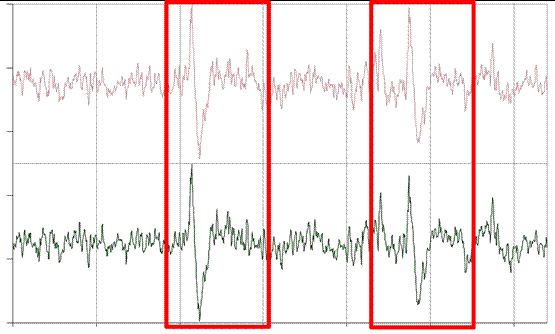
\includegraphics[width=350px]{eyeBlink.png}
  \caption{AF3 and AF4 channel response to eye blink. Credit: \cite{experimenterEPOC}}
    \label{fig:blinkAF}           
\end{figure}

\subsubsection{Affectiv\texttrademark  Suite}
Returns a \texttt{float} between 0 and 1 which describes the power of one of the following emotions:
\begin{itemize}
	\item Engagement/Boredom
	\item Frustration
	\item Meditation
	\item Excitement short term
	\item Excitement long term
\end{itemize}

I have found these emotions to represent quite well my mood. One thing to note is that boredom is not the kind of boredom one feels when they have nothing to do, but it is rather the opposite of engagement, according to Emotiv. See figure for a screenshot of the suite.

The Emotiv User Manual \cite{emotivUserManual} (page 31) provides information on the activities and brainwave types that may trigger each emotion.

\subsubsection{Cognitiv\texttrademark  Suite}
This is probably the most exciting feature of the Emotiv EPOC. Here, you can train 13 actions: push, pull, left, right, lift, drop, 6 rotations (one in each direction for the x, y and z axis) and disappear. The disappear action is more abstract because while the first 12 are real life actions, an object cannot vanish into thin air through whatever methods. The user has to train each action for a period of 8 seconds. This should be done multiple times until an as high as possible skill level is obtained. The more you get used to training, the easier it will become. I have achieved close to 100\% on all 4 actions: push, pull, left, right. At one point, I was able to achieve 100\% on the push action in 5 trainings. The SDK can only detect up to 4 actions at any one time, so one has to choose wisely which actions would be best for their application. See figure \ref{fig:skillLevelMe} for a screenshot of the suite.

\subsubsection{Mouse Emulator (Gyro)}

This data actually comes from a gyroscope fitted in the headset. The original version aims to emulate the mouse movement by changing the head position. Once your head turns to left or right and remains in that position, the centre of the circle becomes your new head position. However, I had access to the Unity 3D plugins and I was able to modify this suite so that the centre of the circle was not recalculated if the head stayed to the left or to the right because I wanted to use the gyro as yet another way to control the car movement. See figure for a screenshot of the suite.

\subsection{Caring for the headset}
The 16 sensors need to be properly hydrated before starting to use the Emotiv EPOC. The hydration is done with contact lenses saline solution which has the purpose of enabling a better transmission of the brainwaves while also sanitising the sensors. First time using the headset may need 15-20 proper hydrations before good contact quality is achieved.

When the user does not expect to use the headset in the next 3-4 days, it is recommended to remove the felt parts from the sensors. Otherwise, the process of oxidation happens more quickly. See figure \ref{fig:cleanVsOxidised} for images of clean sensors and oxidised sensors. The green residue can be cleaned with a cotton swab dipped into a solution of 1/2 water 1/2 white vinegar. If cleaning the interior of the golden plates, take care not to remove the slightly white polymer paste. I have left the felt parts in the sensors when I went on holiday for about 3 weeks. When I returned, the headset was losing contact quality very quickly and after about 15 minutes, it had to be rehydrated. It looks like salt columns may also form in the felt parts. My problem though, was that the golden plates oxidised a lot and after cleaning them as described above I achieved full green sensor contact quality which is the best you can wish for. I firstly cleaned the outside of the golden plates but that did not help too much. Then, I moved to cleaning the inside as well and that did the job for me, although on the Emotiv forums this is not something they would recommend. I was amazed to see the great contact quality I could achieve and it did not have any negative effects on the sensors and they are still in perfect shape 3 months after the cleaning.

\begin{figure}
  \centering
  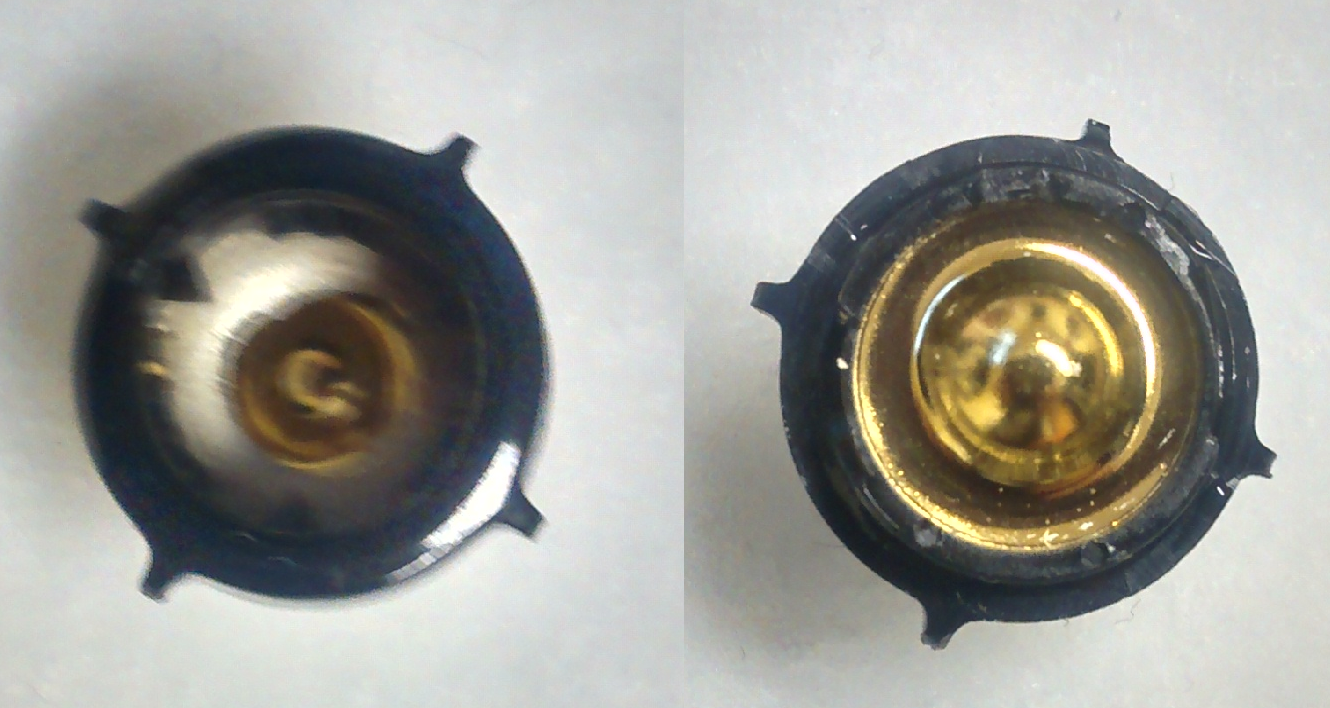
\includegraphics[width=350px]{goodSensorBadSensor.png}
  \caption{From left to right: clean inside of golden plate; clean outside of golden plate; oxidised inside of golden plate; oxidised outside of golden plate.}
    \label{fig:cleanVsOxidised}           
\end{figure}

\subsection{Headset issues}
One of the main problems I encountered is that the wireless connection to the computer is not reliable and it can drop out of the blue. The EPOC+ is now on the market and it seems it might come with a solution for this.

\subsection{EmoComposer}
EmoComposer is a tool which sends simulations of EmoEngine events to an application. This made it easy to test my game without connecting the headset. This was particularly useful in more tricky situations which would have meant spending a long time trying to achieve an action by concentration only.

\subsection{EmoKey}
EmoKey allows mapping of keys to all the interpretations described in this chapter. In this way, one can use the headset to send smiley faces when smiling or laughing for example. One may also use it to paint. These are two of the things that I have tried. It is supposed to be more useful for playing games using the headset. This has been tried in \cite{wowControl} for the \textit{World of Warcraft} game.

\section{Training}
Because training is a difficult part of getting started with the headset, this section is only trying to provide some pointers as to what might work. 

First of all, while training the user should try to keep as still as possible and concentrate on the action being trained. For example, if one is trying to train the push action, the thing which works most of the times is to visualise how the training cube is being pushed to the back of the virtual room. 

Other people find it easy to visualise a flow of energy in the direction of the trained action. 

Repeating words into one's mind does not work. I have seen it working when people say words out loud but the same pace should be kept.

Doing hand gestures works sometimes as \cite{emoTraining} seems to suggest. I have seen one user trying to do this. It worked for a while but then it stopped. Same happened to me.

One thing I have not tried is shifting concentration on the left or right hand side of the body as it is also suggested in \cite{emoTraining}.

Imagining colours or objects for different actions, also does not seem to work.

The problem with training is that there is no `recipe' one can follow. Rather, the user has to try to come up with something that works for them. 

With regards to the training success, in figure \ref{fig:skillLevelMe} you can see one of my achievements. \cite{emoTraining} the fastest learners seem to be young children who believe they can do anything, and very relaxed elderly. In the given example, the father of the poster, aged 82, was able to train reliably the 4 actions in less than 5 minutes. For some notes on how my user testing training worked, read chapter \ref{cha:testing}.

\begin{figure}
  \centering
  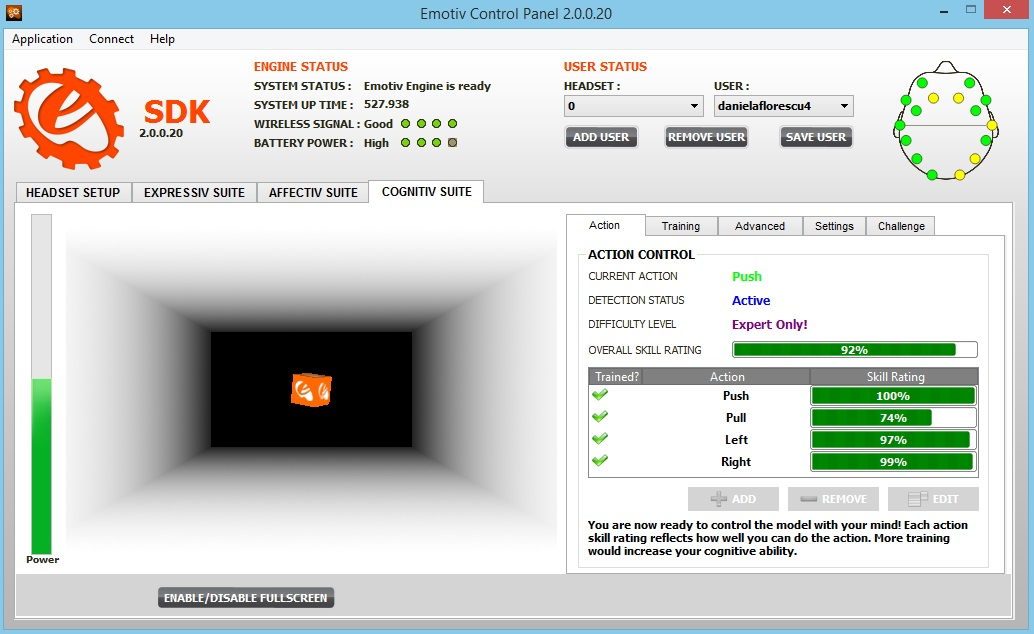
\includegraphics[width=400px]{skillLevel.png}
  \caption{Cognitiv suite training profile}
    \label{fig:skillLevelMe}          
\end{figure}

Some people might encounter difficulties in training the headset. According to \cite{cureBCIilliteracy}, between 15\% and 30\% of the people trying to use a BCI, will not be able to do so. This condition is called `BCI illiteracy' and it better analysed by \cite{BCIilliteracy}. Their study suggests these people have high theta and low alpha waves present across different mental states such as non task related, resting before motor imagery and motor imagery. \cite{cureBCIilliteracy} have tried to come with a solution to this by using a subject-optimised classifier.

\section{Current Applications}
In this section, I am going to have a quick go-through some of the existent applications developed with the help of the Emotiv EPOC.

\begin{itemize}
	\item NeuroPhone \cite{neurophone} is an application which uses the P300 signal and allows the user to scroll through photos of 6 contacts at a time. Once the person the user is looking for is found, the application will dial that person's number.
	\item \cite{handOrthotic} have developed a system which allows the control of a hand prosthetic which opens and closes a patient's hand.
	\item \cite{wheelchairEEG} shows it is difficult to successfully control applications in a highly error sensitive context, such as a wheelchair. 
	\item Mindtunes \cite{mindtunes} is a project in which DJ Fresh has used multiple headsets in order to produce music from the raw EEG data.   
	\item EmoLens \cite{emoLens} tags a user's Flickr photos with emotions and learns to show similar pictures in the future as well as allowing picture search based on the tagged emotion.
\end{itemize}
\chapter{Design}
\label{cha:design}

This chapter describes the design decisions taken in this project and how these work towards achieving the aims described in chapter \ref{cha:intro}.

\section{Overview}
As a methodology used during the project, I have followed the Agile Unified Process. This decision was taken because the process is iterative and it allows the user to be flexible if circumstances change. Agile UP also focuses on producing working code over comprehensive documentation.

For splitting the tasks, I have been using \url{http://trello.com}, a free project management tool which allows you to have virtual boards and cards for each task, making it a virtual Kanban system.

For producing the UML diagrams, I have used \url{http://www.gliffy.com/}, an online tool which allows the user to create 5 diagrams for free.

\subsection{Project workflow}
The project has consisted of 4 phases:
\begin{itemize}
	\item \textbf{Phase 1} consisted of initial project documentation, background reading and an attempt to build a 3D car model to be used during the game. The sides of the car model were realistic enough, but I could not figure out how to build the front and the back, so I have used 3 free 3D models that I have found online. See Appendix for the sources of these objects.
	\item During \textbf{phase 2}, I have learnt more about Unity by following the \cite{walkerboys} tutorial. Following that, \cite{flattutorials} was a good starting point to how one can create a car game in Unity. Some more advanced car physics ideas were inspired from \cite{carphysics}.
	\item \textbf{Phase 3} has seen the start of implementing the functionality from the developer's API of the Emotiv EPOC. The most important part was getting the training working inside the game.
	\item In \textbf{Phase 4} the main concern was improving the user experience, getting some user testing done and allowing the player a choice of car models and colours.
\end{itemize}

\subsection{Requirements}

\subsubsection{Functional requirements}
In the final game, the player should be able to: 
\begin{itemize}
	\item Create/Delete/Change a player profile;
	\item Train the headset for neutral, push, pull, left, right states;
	\item Allow the user to accept/reject/reset a training session;
	\item Display the updated skill level after each training session;
	\item Provide visual feedback as to how well the training is going through an animated object;
	\item Alert the user in the training scene if a training profile is not complete;
	\item Display the top 10 highest scores for Keyboard mode play and Cognitiv mode play;
	\item In the Options tab, allow the user to change sound volume, sound effects volume and whether the game will be played in fullscreen;
	\item Allow the user to change between Keyboard, Cognitiv and Gyro play modes;
	\item Provide instructions to train and play the game;
	\item Pause/Exit the game;
	\item Allow the selection of a car model and colour;
	\item Race yourself during the game play.
\end{itemize}

\subsubsection{Non-functional requirements}
\begin{itemize}
	\item The game should be portable (i.e. playable on multiple operating systems);
	\item Once loaded, there should be no long waiting periods of time.
\end{itemize}

\subsection{Separation of concerns}
The Model-view-controller architecture has been used with the purpose of separating the concerns such that the controller (the script) is manipulating the model (car or environment) which then updates the view (the user interface).

\section{Design Patterns}

\textbf{Abstract Factory} has been used to create cars from the abstract \texttt{Car} class. \texttt{AudiR8} and \texttt{FerrariCalifornia} are thus inheriting from \texttt{Car}. See figure \ref{fig:classDiagram} for the UML class diagram.

\textbf{Strategy} is used to decide which car control options to follow depending on the game play mode: Keyboard, Cognitiv or Gyro. It is also used in the car model choice.

\begin{landscape}
\pagestyle{plain}
\begin{figure}
  \centering
  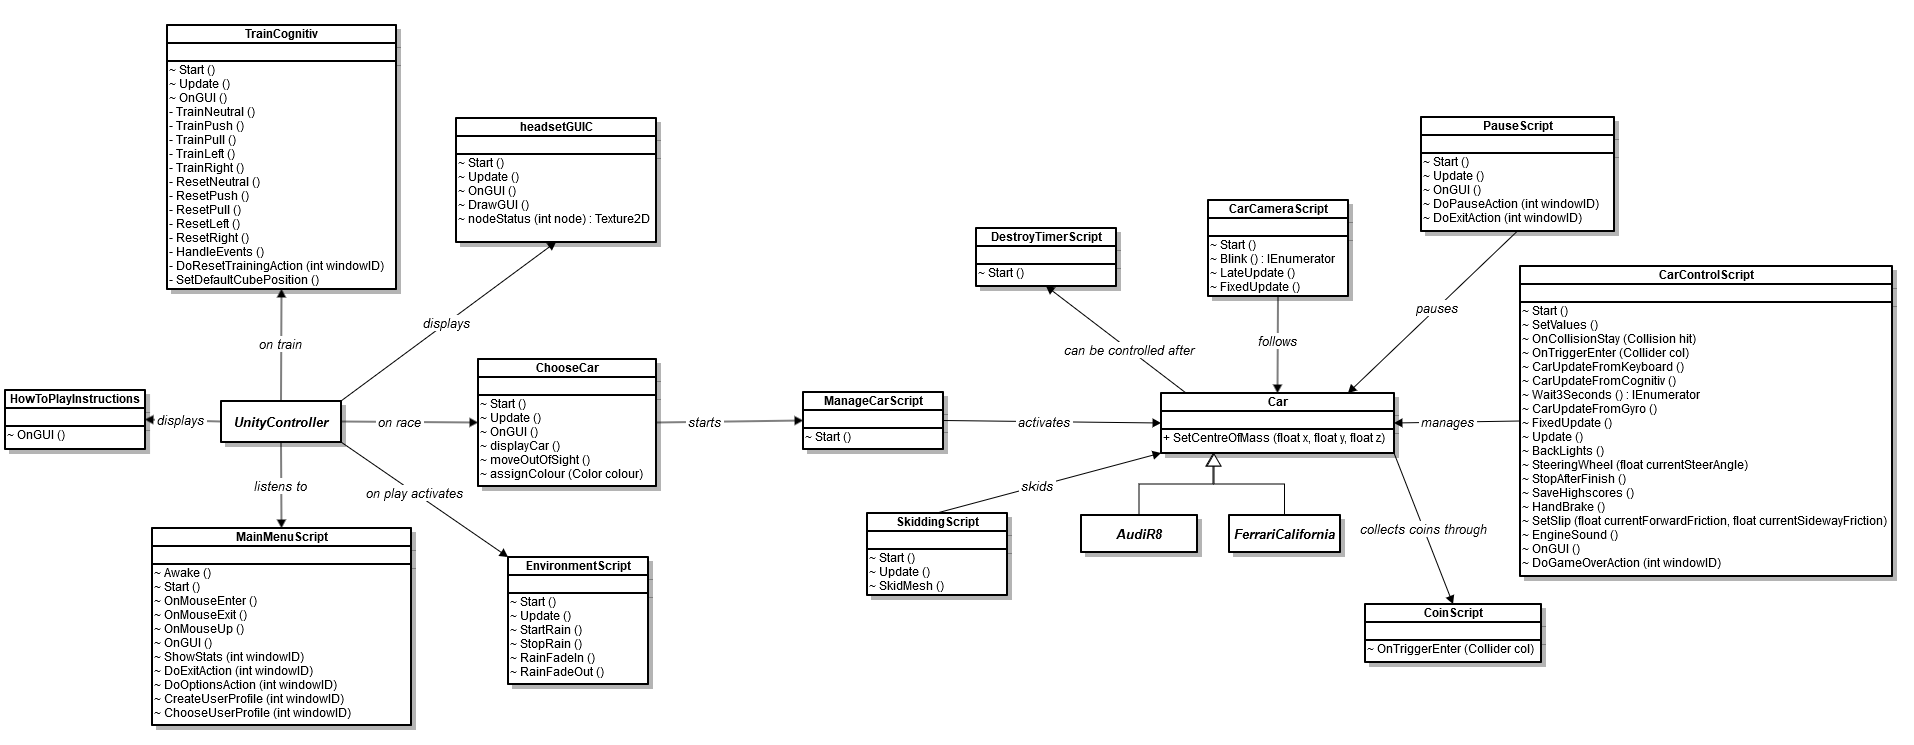
\includegraphics[width=750px]{CogniDriverDomainClassDiagram.png}
  \caption{Domain class diagram for CogniDriver. The instance variables have been omitted for simplification.}
    \label{fig:classDiagram}           
\end{figure}
\end{landscape}
\pagestyle{fancy}

\chapter{Implementation}
\label{cha:implementation}

This chapter presents the main implementation details during the development phase of the project.

\section{Interfacing with Emotiv}
The Unity 3D plugin package from Emotiv comes in a suite of 11 C\# files which we will describe in a bit more detail. In order to get access to this data, an  \texttt{EPOCManager} object was created. This object contains all the plugins in the package apart from  \texttt{EdkDll}, \texttt{EmoState}, \texttt{EmoProfileManagement} and \texttt{LabelDraw}. In the following subsections, we are going to provide some very short code snippets since these might prove useful in the future for someone wishing to develop a game using Unity and Emotiv.

\subsection{EdkDll}
Contains the implementation of the Emotiv API.

\subsection{EmoAffectiv} 
This class gives access to the player emotions described in Section \ref{part:affectiv} through calls that directly access one of the public instance variables. For example,

\begin{Verbatim}[frame=single, framesep=3mm]
EmoAffectiv.frustrationScore
\end{Verbatim}

returns a value representing how frustrated the user is.

In CogniDriver, frustration is used to get the rain started once the score is higher than 50\% and the excitement is lower than 50\%. 

\subsection{EmoCognitiv} 
It is a class containing methods to start or reset the training. It automatically handles events which start, reset, erase, declare successful or failed training. We have added accessor methods to obtain the current action, its power and the trained actions. We have also added a GUI method, \texttt{DoTrainingCompleteAction(int windowID)} which pops up the window asking the user whether the training should be accepted or rejected and it handles the response appropriately. Before starting the training though, the 4 actions (push, pull, left, right) have to be activated through a call such as: 

\begin{Verbatim}[frame=single, framesep=3mm]
EmoCognitiv.EnableCognitivAction(EmoCognitiv.cognitivActionList[6], 
				true);
\end{Verbatim}
		
where 6 represents the index of the \textit{right} action. At the end, the list of 4 actions has to be set through a call to 

\begin{Verbatim}[frame=single, framesep=3mm]
EmoCognitiv.EnableCognitivActionsList();
\end{Verbatim}

The skill for the \textit{push} action is obtained as follows:

\begin{Verbatim}[frame=single, framesep=3mm]
Single pushSkill = EmoEngine.Instance.CognitivGetActionSkillRating(
			(uint)EmoUserManagement.currentUser,
			EmoCognitiv.cognitivActionList[1]); 
\end{Verbatim}

\subsection{EmoEngine}
`Is the logical abstraction of the functionality that Emotiv provides in edk.dll.'\cite{emotivSDKUserManual}

\subsection{EmoEngineInst}
It is used most often to change the connection method from live data to simulated data (through the use of EmoComposer (subsection \ref{part:emocomposer})).

\subsection{EmoExpressiv}
The EmoExpressiv class is useful in order to get access to the player's facial expressions through simple calls to the public instance variables, such as the following which checks whether the player did a left wink:

\begin{Verbatim}[frame=single, framesep=3mm]
EmoExpressiv.isLeftWink
\end{Verbatim}

In CogniDriver, left wink is used to change the camera view. Clenching teeth will action the car's handbrake. 

\subsection{EmoGyroData}
Gives access to the head position in relation to the circle observed in figure. One may also obtain the \texttt{x} and \texttt{y} coordinates of the gyro. However, we could not find the maximum and minimum values, nor are there 2 online references which give the same numbers.

\subsection{EmoProfileManagement}
This class is useful to handle the player profiles. In CogniDriver, we have limited the number of player profiles to 10 because of the following reasons:
\begin{itemize}
	\item The training for a saved profile can take a few MB;
	\item Unity does not contain a drop down list as a GUI element;
	\item Unity does not allow overflow of windows.
\end{itemize}

When the game starts, the list of user profiles (files saved with the \texttt{.up} extension) is loaded through a call to:

\begin{Verbatim}[frame=single, framesep=3mm]
EmoProfileManagement.Instance.LoadProfilesFromFile();
\end{Verbatim}

A new profile is added by calling:

\begin{Verbatim}[frame=single, framesep=3mm]
EmoProfileManagement.Instance.AddNewProfile(playerName);
\end{Verbatim}

An existing profile is deleted by calling

\begin{Verbatim}[frame=single, framesep=3mm]
EmoProfileManagement.Instance.DeleteProfile(selectedPlayer);
\end{Verbatim}

Profile data is saved after training by a call to 

\begin{Verbatim}[frame=single, framesep=3mm]
EmoProfileManagement.Instance.SaveCurrentProfile();
\end{Verbatim}

followed by

\begin{Verbatim}[frame=single, framesep=3mm]
EmoProfileManagement.Instance.SaveProfilesToFile();
\end{Verbatim}

On selection of a profile, this is set by calling

\begin{Verbatim}[frame=single, framesep=3mm]
EmoProfileManagement.Instance.SetUserProfile(selectedPlayer);
\end{Verbatim}

\subsection{EmoState}
Represents the emotional status of the user at a given time \cite{emotivSDKUserManual}. This class is used by \texttt{EmoAffectiv}, \texttt{EmoExpressiv} and \texttt{EmoCognitiv} mainly. We did not need to call any functions directly from this class.

\subsection{EmoUserManagement}
Keeps track of the current user, the current number of user profiles and also fires events when a USB dongle is inserted or removed. We did not need to use this class directly apart from obtaining the current user by calling

\begin{Verbatim}[frame=single, framesep=3mm]
EmoUserManagement.currentUser
\end{Verbatim}

\subsection{LabelDraw}
We did not need to use this class while developing CogniDriver.

\section{Scene description}
In Unity, a scene contains all the objects for a part of the game such as a level or a different screen. For CogniDriver, we have split the game in 6 scenes. All of the scenes, apart from the splash screen, will display the sensor contact quality, current action and the power of the current action. This can be observed in figure \ref{fig:mainmenuscene}.

See figure \ref{fig:sceneInteraction} for an example of how the scenes interact with each other.

\begin{figure}
  \centering
  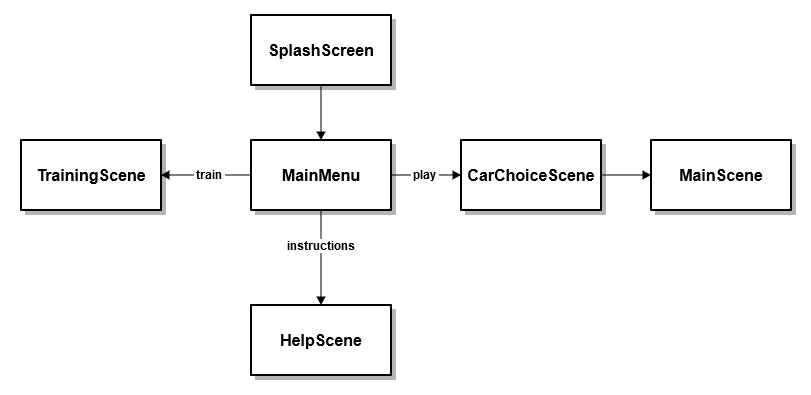
\includegraphics[width=450px]{sceneInteraction.png}
  \caption{Scene interaction diagram from the moment the application starts loading.}
    \label{fig:sceneInteraction}           
\end{figure}

\subsection{CarChoiceScene}
The purpose of this scene is to allow the player to choose a car model and colour. At the moment, we have used only 2 car models. I had three of them in mind but one of the models did not allow modifications to the grouping of its components. Figure \ref{fig:carchoicescene} shows how this looks like in the game.

\begin{figure}
  \centering
  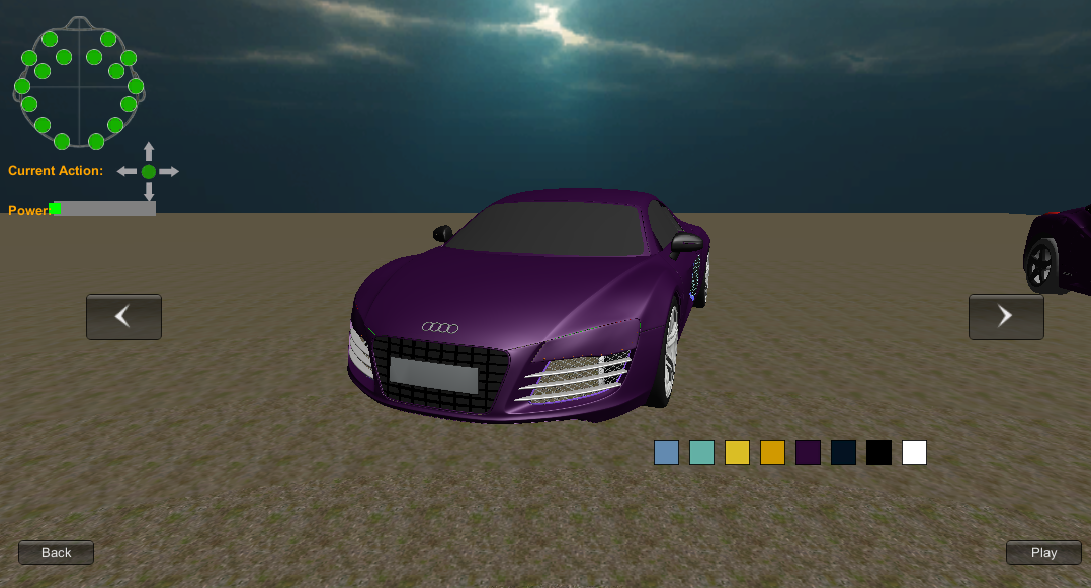
\includegraphics[width=400px]{carchoicescene.png}
  \caption{Car choice scene}
    \label{fig:carchoicescene}           
\end{figure}

\subsection{HelpScene}
Contains simple instructions describing how the game is to be played. 

\subsection{MainMenu}
This scene allows the player to:
\begin{itemize}
	\item manage the player profiles;
	\item start the race;
	\item train a player profile to be played in Cognitiv mode;
	\item see the highscores for Keyboard and Cognitiv mode in the \textit{Statistics} tab;
	\item read instructions about training and playing the game;
	\item adjust the sound effects and music volume, fullscreen enabling and select the play mode;
	\item exit the game.
\end{itemize}

Figure \ref{fig:mainmenuscene} shows an example of how the main menu scene looks like.

\begin{figure}
  \centering
  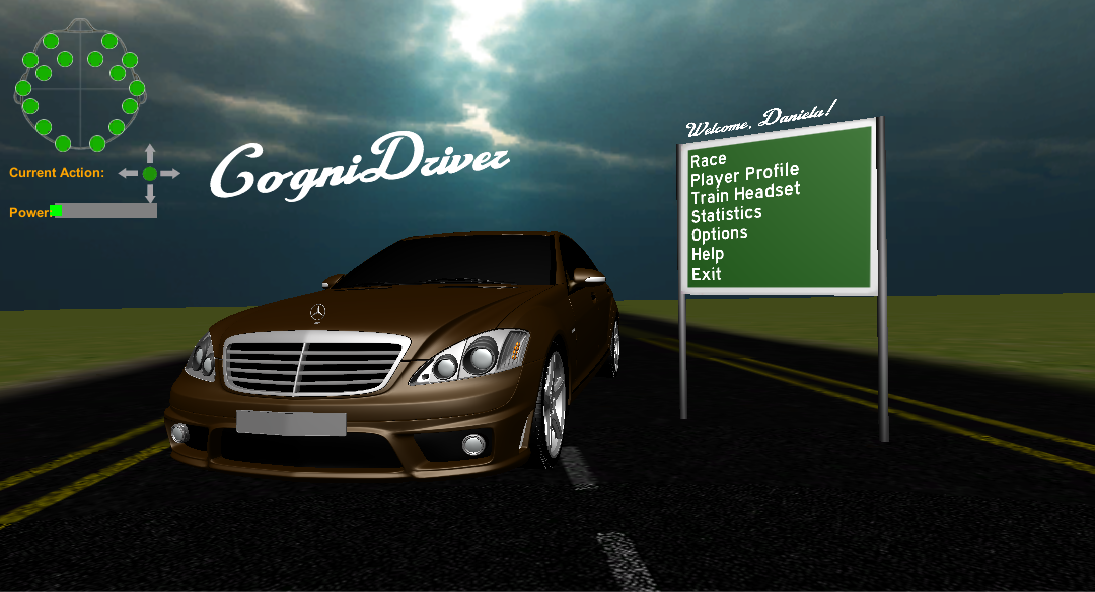
\includegraphics[width=400px]{mainmenuscene.png}
  \caption{Main menu scene}
    \label{fig:mainmenuscene}           
\end{figure}

\subsection{MainScene}
This is the proper game play where the player is controlling the car around the track. It can be observed in figure \ref{fig:mainscene}.

\begin{figure}
  \centering
  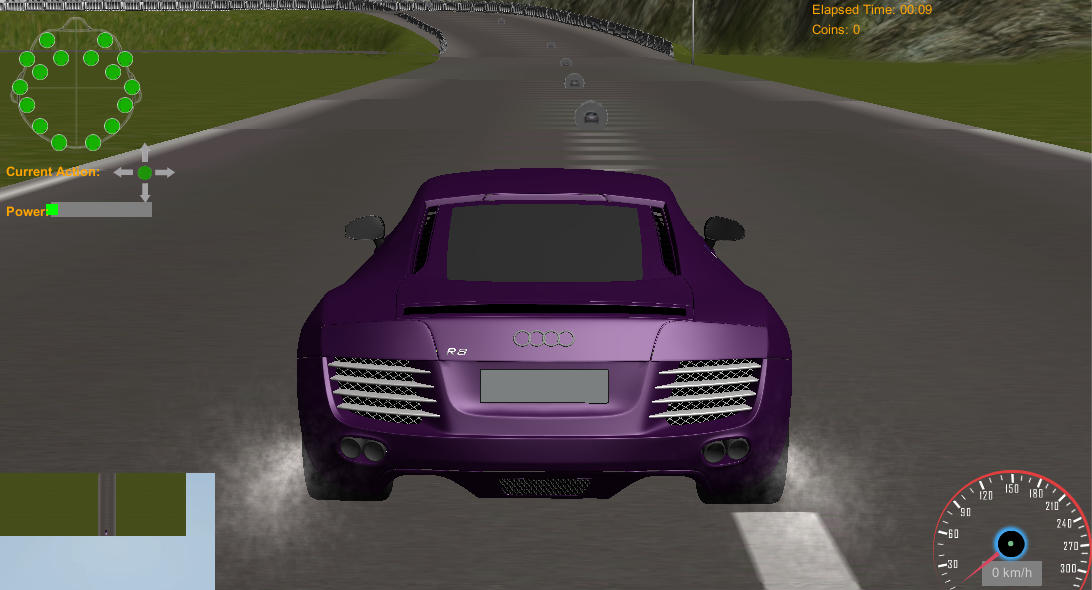
\includegraphics[width=400px]{mainscene.png}
  \caption{Main scene}
    \label{fig:mainscene}           
\end{figure}

\subsection{TrainingScene}
Its aim is to provide a place where the player can train the 5 actions: neutral (staying relaxed), push, pull, left, right. The training may also be reset for each action in turn. The user will receive visual feedback from the animated car on how well the training has been done. A screenshot can be observed in figure \ref{fig:trainingscene}.

\begin{figure}
  \centering
  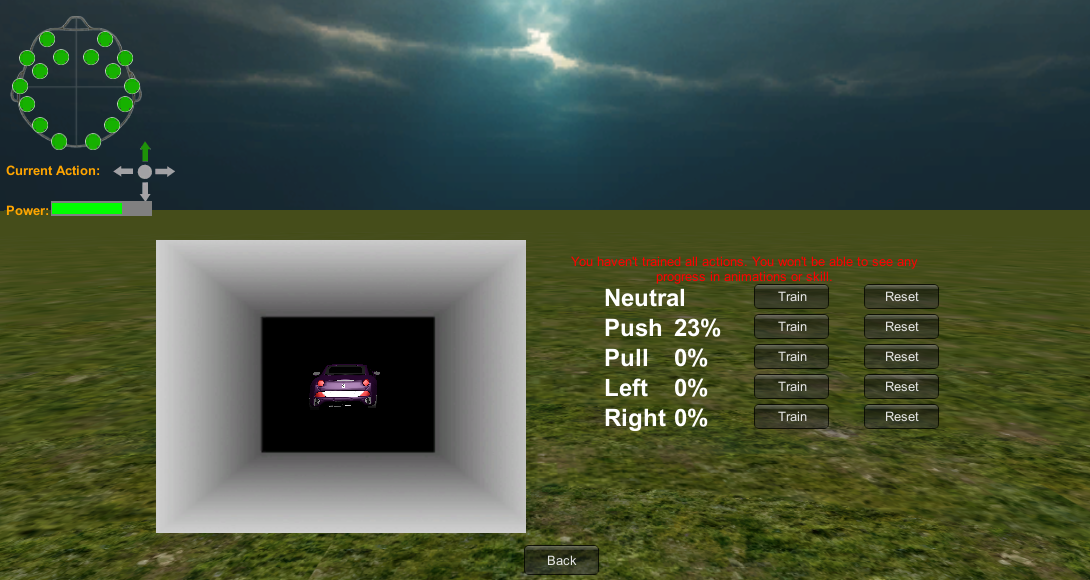
\includegraphics[width=400px]{trainingscene.png}
  \caption{Training scene}
    \label{fig:trainingscene}           
\end{figure}

\section{Notes}

We took the decision of having the Cognitiv training done inside the game so that a new player would not need to open another application, for example the Emotiv Control Panel, in order to train the profile.

For passing variables between different scenes, Unity's \texttt{PlayerPrefs} module has been very useful. One example of its use is in saving the highscores. We will go in a bit more detail about what the saving highscores process is.
\begin{enumerate}
	\item Get the current number of entries in the highscore list.
	\item If it is \textgreater  10, check if current entry is better than existing ones. If it is, record it.
	\item A top 10 value is stored as: 
	
	\begin{Verbatim}[frame=single, framesep=3mm]
key = topKeyPrefix;
value = String(PlayerName;elapsedTimeInSeconds;coins)
	\end{Verbatim}
	\item The entry is a fraction of the elapsed time in seconds and the number of collected coins.
	\item Find the position where the new entry should be inserted.
	\item Shuffle previous entries if necessary.
	\item Finally, insert the new value and update the number of entries in the highscores table.
\end{enumerate}

The user has access to some screen helpers during the time they are playing the game. These are:
\begin{itemize}
	\item[-] a speedometer which displays the current speed in both analog and digital mode;
	\item[-] a square minimap which shows where the car is placed on the map when it is seen from above;
	\item[-] the elapsed time since the start of the game;
	\item[-] the number of coins collected.
\end{itemize}

\subsection{Gyro mode}
Playing the game while using the headset's gyroscope is doable. However, most of the times the user is getting eyes off the screen meaning they may not see where and how the car is moving. 

\chapter{Testing and evaluation}
\label{cha:testing}

The initial plan was to have a total of 10 participants to take part in a 2-hour testing process. However, some people dropped out while other people expressed interest, so the final number of participants was 13. All the participants were university students. The testing took place in week 4 of second semester, more precisely 17th to 20th of February.

At the time of user testing, the game was finished with the exception of the car model and colour choice.

In this chapter, we are going to discuss the results of the user testing. The used questionnaire can be found in Appendix \ref{appendix:userStudy}. 

For the purposes of testing the projects, the participants were firstly asked to play the game in keyboard mode. Following this, they were asked to fill in a NASA TLX (Task Load Index) test so that we would have a measurement of how demanding this task was for the user. Next, the Emotiv EPOC headset was fit on the participant's head and the training process would begin. After feeling confident enough for the first action (push), the user could see it working in the actual game play. We insisted on properly training 2 actions: push - for acceleration - and left - for a left turn. The reason why left was necessary is because the track does a left turn on a slightly elevated terrain. Less than 5 users have probably had enough time to train the other 2 states (pull and right) as well. Again, after the 2 hours were almost up, the participant was asked to take another NASA TLX test, this time taking into account how demanding the process was for Cognitiv game play. Finally, the participant was asked to fill in the user study questionnaire in Appendix \ref{appendix:userStudy}. 

The following sections will describe the results of the user testing. In Section \ref{section:implemented}, we will highlight what was changed in CogniDriver following the participants' answers, in the period of 2 weeks left before the project demonstrations period begun. Figure \ref{fig:testing} shows one of the trained user profiles during testing.

\begin{figure}
  \centering
  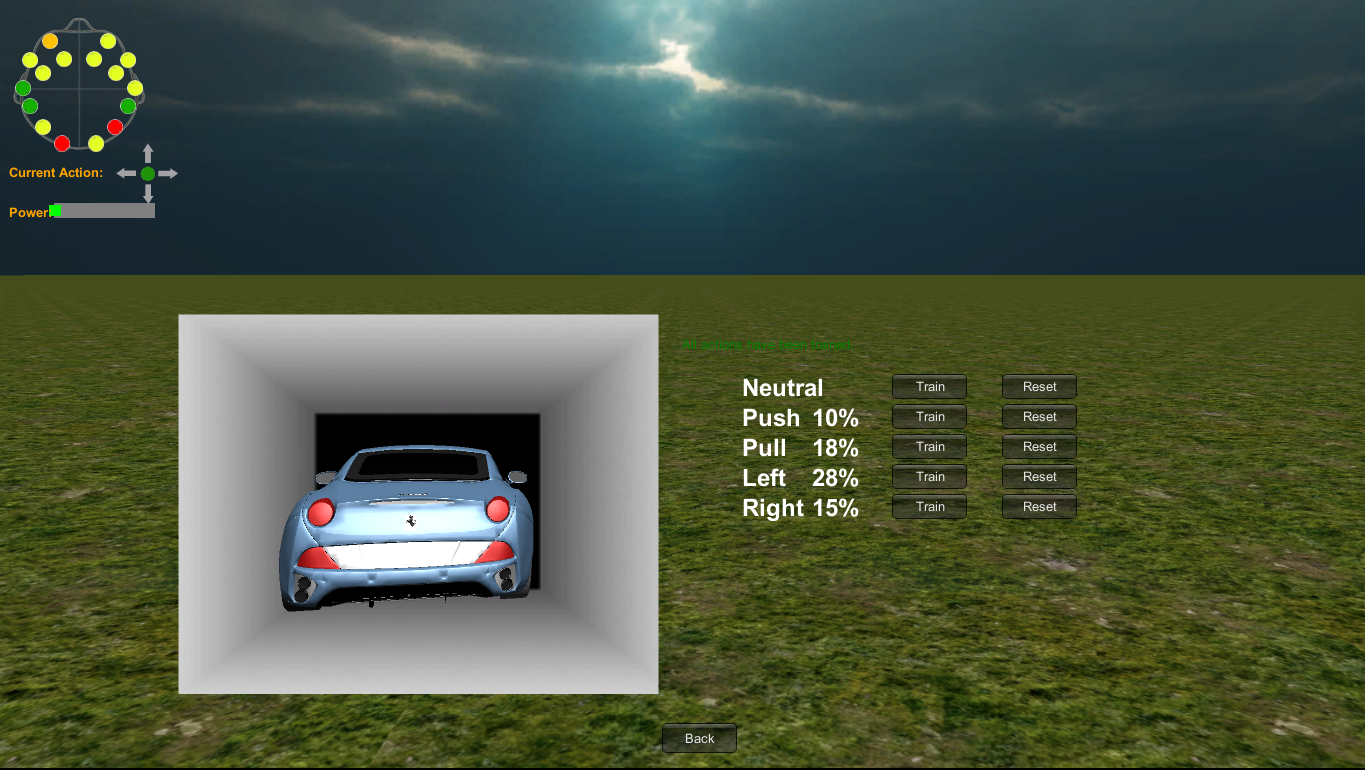
\includegraphics[width=400px]{lloyd.png}
  \caption{Trained user profile during user testing}
    \label{fig:testing}           
\end{figure}

\section{Observations}

Some of the participants displayed better skill in training the headset if the testing was done in the morning. This is compared to evenings, when some of the partipants complained about being tired and not being able to concentrate properly.

The testing was done using a cube as the training object. In my opinion, this would have made training consistent with people used to the Emotiv EPOC Control Panel or other applications which require Cognitiv training. 

It may be difficult to switch to a different mental state when training a new action. As a result, new training data for an action, might override data for a previous action. This happened to me a few times and it did happen with some of the participants as well.

When training or playing the game, if the car is being moved, the enthusiasm generated by that may make the player lose concentration.

\section{NASA TLX results}
The test was taken using the \cite{nasatlx} online version developed by Keith Vertanen. It produces the analysis of the input data for each person at the end of the test. 

For keyboard mode, the overall mean difficulty was 51.611\% with a standard deviation of 17.494\%.

For Cognitiv mode, the overall mean difficulty was 90.571\% with a standard deviation of 13.964\%.

This tells us the participants have found the game much easier to play in keyboard mode compared to Cognitiv mode which was very demanding.

\section{Analysis of user questionnaire answers}
The user questionnaire aimed to measure things such as the comfort of wearing the headset and how demanding the training and playing were, especially in Cognitiv mode.

The mean of the comfort of wearing the headset was 5.692 out of 10 with an approximately equal spread of scores. Most of the participants have started feeling the discomfort after 20-40 minutes of wearing the headset. 

For the questions regarding the demand of the process, the participants' scores were quite unanimous. The training demand obtained a score of 4.23/10, the play demand obtained a score of 3.153/10 and the ease demand obtained 2.153/10. The similarity between the keyboard play and Cognitiv play was of 2.307/10 suggesting the two modes are not similar.

\section{Good points about the game}
The first point to make was that users found it easy to focus on the task because driving is a real life skill and it is easy to understand. Many times, participants made correlations between the driving game and the real life skill.

Raining when frustrated was considered a great feature by most.

The graphics were generally appreciated and feedback was received on the track as being sensible. 

Some players enjoyed the funny game physics because there were opportunities for cheating. However, these opportunities have been reduced now and we have tried improving the physics so that not as much skidding would occur.

The training interface was considered clear and understandable.

\section{Bad points about the game}
It was hard to tell which way is the right direction of driving if the car skid and the player got disorientated.

The car accelerated too fast and some of the game physics were peculiar. 

Some considered it would have been useful to see the brainwaves for each channel since this might have provided more feedback on how the training was going and how to concentrate on completing the task.

The training process requires concentration and it can take a long time. Some people were disturbed by the amount of clicking going on in order to start training, accept or reject it and then start again. It also got the participant distracted and it was breaking the concentration level. Sometimes, I would do the clicking for the participant so I could catch the events when the object was really being moved. Complaints were received regarding the training as being too stressful, frustrating and not rewarding. The amount of clicking, although disliked by many, is not something which could be changed since the training process can vary in duration. It was suggested that an approach to this might be to automatically accept a training if it meets some set guidelines but then the participant is quite out of control of the process. In addition, it might make the movement more difficult to control.

Some invisible colliders from around the mountains were slightly touching the road side. This has now been fixed. A collider is an invisible object that is used either as a barrier to stop another object from going through it or which is used as a trigger to detect whether another object has reached that point.

The driver seat view was not always enjoyable, especially when the sensor contact quality was not perfect and the blink would be mistaken for a left wink which would then cause the camera view to change.

\section{What should be improved and what has been implemented?}
\label{section:implemented}
It has been suggested by more than a half of the participants that training would be easier if it was done with a car object rather than a cube as this made them more properly visualise the action. It also made it easier to activate an action while playing the game. This has been implemented.

Checkpoints were another suggestion so that players could be stopped from cheating and taking a short route to the finish line. This has been implemented with the help of invisible colliders which were being triggered when the car would pass through them. A total of 17 checkpoints have been inserted. At the finish line, if the number of checkpoints the player has been through is different than 17, the message in figure \ref{fig:ohno} will appear, offering the option to restart the game.

\begin{figure}
  \centering
  
\includegraphics[width=300px]{ohno.png}
  \caption{A print screen of the message which will occur in case the player tries to follow a shortcut to the finish line}
    \label{fig:ohno}        
\end{figure}

The current action used to be displayed as text, but the suggestion was to have a system of arrows being highlighted for each type of movement. This has been implemented.

One suggestion was to add some coins to the road that the player could collect. This has been implemented and it solves the issue of the users not knowing which is the right direction of going. It also obliges the player to stick more to the centre of the road and it provided an extra way of deciding the highscores, besides the elapsed time.  

There used to be a quite annoying reverse sound which was suggested to be removed by the majority of participants. It was seen as distracting when the player was trying to concentrate on the action. The motor sound though, did not seem as stressful.

There used to be no way of restarting the race from the keyboard. This is now done when the player is pressing the 'R' key. Also, using 'T' will make the car respawn at the last checkpoint it has been through just in case the player gets lost around the environment. It is not something that should happen too often, but it might occur.

The things which have not been implemented had to do with not having access to the raw EEG data or them simply not being feasible or important.

From a talk after the testing session was complete, it was suggested it would be good to give the car different speeds on grass and road. This has been implemented. The car accelerates about 2 times slower when it gets on the grass area.
\chapter{Conclusions}
\label{cha:conclusions}
This chapter will describe what I have learnt, what I could have improved and some final thoughts about the project.

\section{Personal development}
Before starting this project, I have not been programming in C\# nor did I have any experience in working with Unity. Every time I try a new programming language or technology, I get a confidence boost because I see I can handle the situation and the experience will be beneficial in my future career. What I wish I had done about Unity, was to check the default access modifiers, especially for methods. Also, the order of the things in the \texttt{Update} function might matter. 

An application should be designed with software design patterns in mind. This will make it more secure and it will careful consideration on behalf of the developer. 

Documentation is important since other people might need to continue your work or they might want to adjust certain parts in order to fit their purposes.

It is useful to keep a logbook of the work one is doing and to write down the problems they encounter. This will provide a good retrospective about the things they have learnt or they should improve for the next application.

It is important to use suitable names at all times.

\section{Summary}

Nowadays, we have exercised using the keyboard for long periods of time, so it seems easier to control a game in this mode, but if we put more practice into playing with an EEG and properly training the Cognitiv suite, we could achieve same results with much less of an effort. \cite{moviebrain} shows it is possible to use an fMRI (functional magnetic resonance imaging) to see quite similar pictures with what the participant is seeing while watching a movie. Given this, in a relatively short period of time, brain devices may be able to read one's mind.

My personal feeling about this project is that is helped me see on my skin how design decisions affect the development of an application. In addition, the more time passes from a bad decision, the longer it will take to fix it. I am happy to think that my next project will benefit from the lessons learnt here and I also hope the views I have provided in this report will be helpful to other people with similar circumstances.

At the time of this writing, the full application source code and executable binary are available at \texttt{https://github.com/florescu/CogniDriver}.

\nocite{jmurray}
\chapter{Conclusions}
\label{cha:conclusions}

\section{Achievements}

\section{Personal development}

\section{Further work}

\section{Summary}

\bibliography{refs}             % this causes the references to be
                                % listed

\bibliographystyle{apalike}       % this determines the style in which
                                % the references are printed, other
                                % possible values are plain and abbrv
%% Appendices start here
\appendix
\chapter{Example of operation}

An appendix is just like any other chapter, except that it comes after
the appendix command in the master file.

One use of an appendix is to include an example of input to the system
and the corresponding output.

One way to do this is to include, unformatted, an existing input file. 
You can do this using \verb=\verbatiminput=. In this appendix we
include a copy of the C file \textsf{hello.c} and its output file
\textsf{hello.out}. If you use this facility you should make sure that
the file which you input does not contain \texttt{TAB} characters,
since \LaTeX\ treats each \texttt{TAB} as a single space; you can use
the Unix command \texttt{expand} (see manual page) to expand tabs into
the appropriate number of spaces. 

\section{Example input and output}
\label{sec:inp-eg}
\subsection{Input}
\label{sec:input}
(Actually, this isn't input, it's the source code, but it will do as
an example)

%\verbatiminput{hello.c}

\subsection{Output}
\label{sec:output}

%\verbatiminput{hello.out}
\subsection{Another way to include code}
You can also use the capabilities of the \texttt{listings} package to
include sections of code, it does some keyword highlighting.

%\lstinputlisting[language=C]{hello.c}

% Local Variables: 
% mode: latex
% TeX-master: "report"
% End: 

\chapter{CogniDriver - 3D Object Sources}
\label{appendix:3dobjects}

Below is a list of all the 3D objects that have been imported in the game:


\begin{table}[h]
                             
\begin{tabular}{| c |m{10cm} | }
\hline
\textbf{Image}  & \textbf{Source} \\ \hline
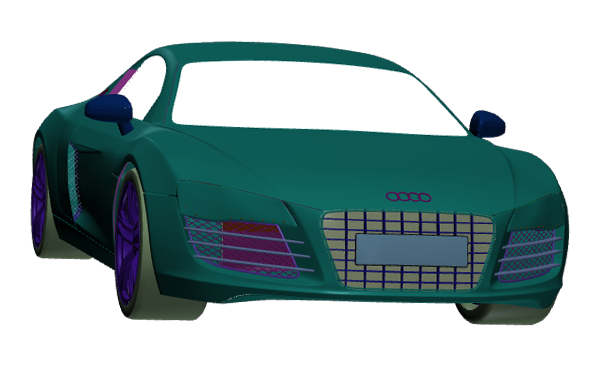
\includegraphics[height=50px]{audir8.png}    & \url{http://tf3dm.com/3d-model/audi-r8-69023.html}    \\ \hline
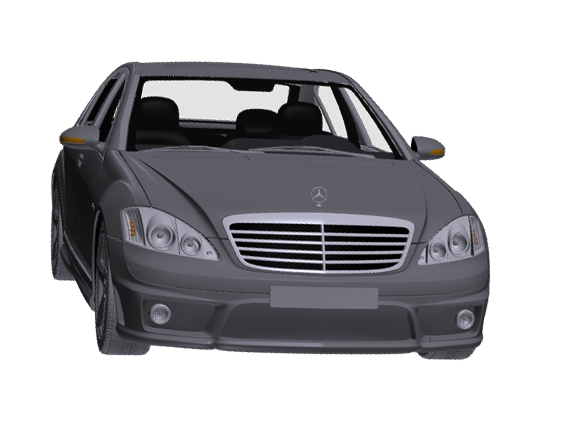
\includegraphics[height=50px]{mercedes.png}    & \url{http://archive3d.net/?a=download&id=8c488f86}    \\ \hline
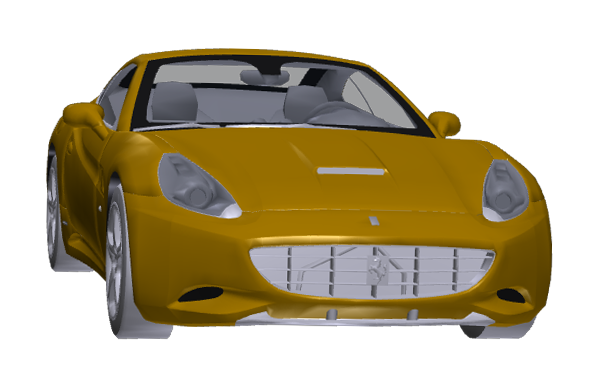
\includegraphics[height=50px]{california.png}    & \url{http://www.mediafire.com/download/cdbb5neezcva198/California.zip}    \\ \hline
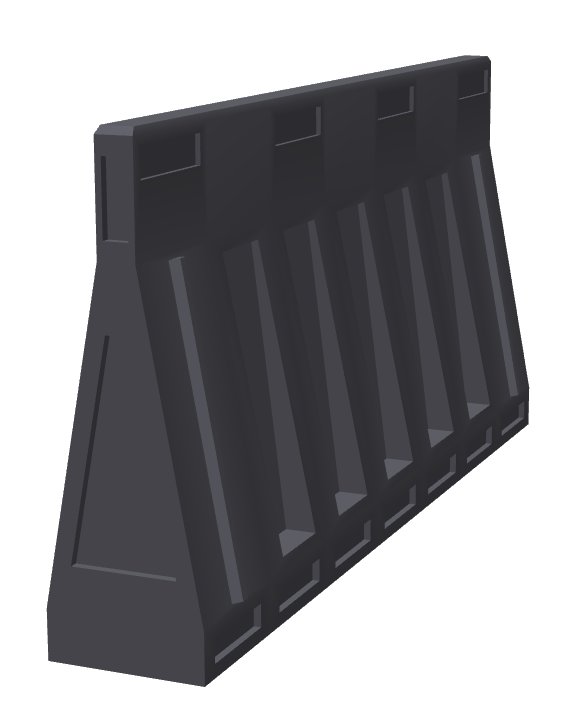
\includegraphics[height=50px]{fence.png}    & \url{http://www.archibaseplanet.com/download/dc2c3978.html}    \\ \hline
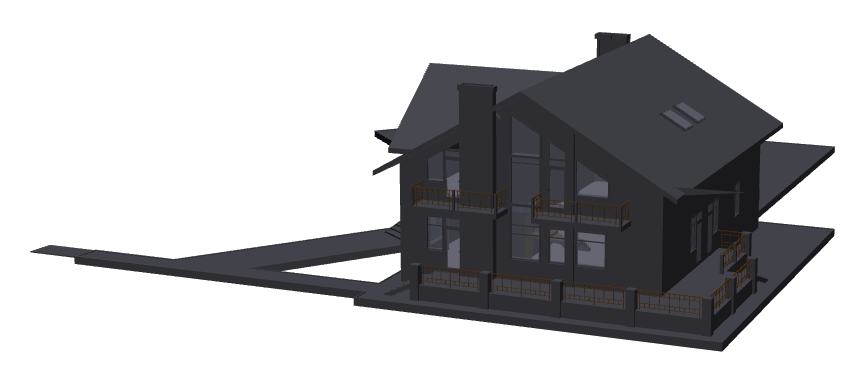
\includegraphics[height=50px]{house.png}    & \url{http://tf3dm.com/3d-model/house-10483.html}    \\ \hline
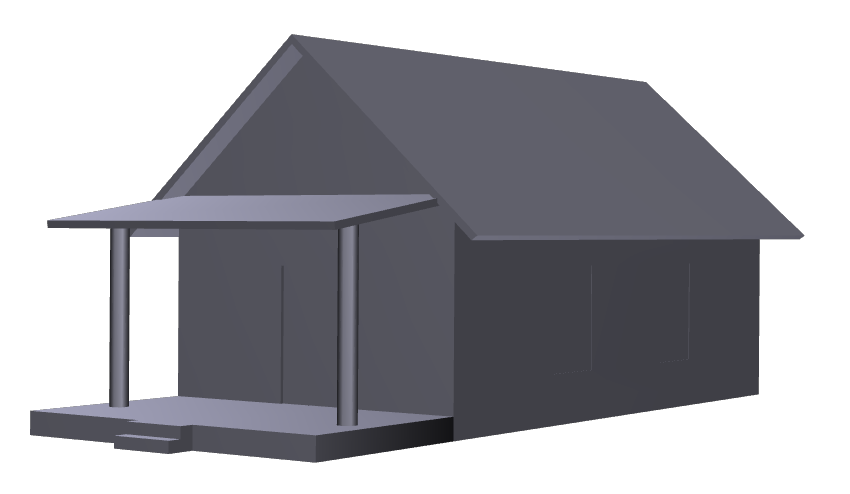
\includegraphics[height=50px]{farmhouse.png}    & \url{http://tf3dm.com/3d-model/old-farm-house-91130.html}    \\ \hline
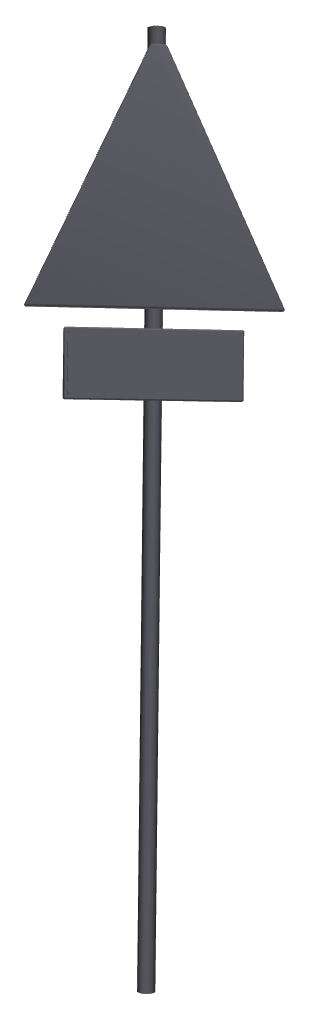
\includegraphics[height=50px]{roadsign.png}    & \url{http://archive3d.net/?a=download&id=6d06cd33}    \\ \hline
\end{tabular}
\end{table}

\end{document}
